\documentclass[a4paper]{article}

\usepackage[english]{babel}
\usepackage[utf8x]{inputenc}
\usepackage{amsmath}
\usepackage{graphicx}
\usepackage[colorinlistoftodos]{todonotes}
\usepackage{fullpage}
\usepackage{amsfonts}
\usepackage{hyperref}
\usepackage{url}

\title{Report of Project: Forward-Planning Agent}
\author{Israel G. de Oliveira}
\date{January 6, 2019}
\begin{document}
\maketitle

\section{Introduction}
This report is about the building a Forward-Planning Agent, project part from Artificial Intelligence Nanodegree \cite{githubUdacityAIND}. The objective is implement functions to able a agent to solve planning problems based on symbolic logic and classical search (progression search), doing experiments with different search algorithms and heuristics \cite{githubUdacityAINDProj2}. This project is based on book Artificial intelligence: a modern approach \cite{russell2009artificial}.

\subsection{Planning Problems}

The planning problems used is based on the example Air Cargo Problem, 10.1.1 from \cite{russell2009artificial}, with four sized variants \cite{githubUdacityAINDProj2}, in according with the Table \ref{airps}. 

\begin{table}[htpb]
   \caption{ Air Cargo Problems}
    \label{tab:cronograma}
    \centering
        \begin{tabular}{ c | c | c | c}
           Problem nº & Planes & Cargos & Airports \\\hline
           1          & 2      & 2      & 2 \\
           2          & 3      & 3      & 3 \\
           3          & 2      & 4      & 4 \\
           4          & 2      & 5      & 4 \\\hline
        \end{tabular}
        \label{airps}
\end{table}

One way to solve this problems is use a graph representation connecting all logic literals and possible actions. With a graph, it is possible to use a search algorithm to find a solution \cite{russell2009artificial}. Not only, for some search algorithms, it is possible to use a heuristic method to estimate the cost for each action (connection in graph), in some cases, improving the finding for a solution (less time expending on searching).

\subsection{Search Algorithms}

The search algorithms proposed to use are Breadth First Search (BFS), Depth First Graph Search (DFS), Uniform Cost Search (UCS), Greedy Best First Graph Search (GBFGS) and A* Search \cite{githubUdacityAINDProj2}. All this algorithm is already implemented with the framework provided by Udacity, available in \cite{githubUdacityAINDProj2}.

BFS is a instance of the tree search with FIFO (First In, First Out) queue. This algorithm is complete (completeness aspect). The solution is not necessarily optimal: because when a objective node is found at a (depth) level $d$ it is not necessarily the best objective node. The total new nodes is $O(b^d)$ with $b$ successors. 

Considering the same step cost 1 for all nodes, we have the BFS. For achieve the UCS, we do a extended version considering a step cost function $g(n)$, for a $n$-node, then is possible to achieve a optimal solution. Basically, expanding the node with the lowest cost. There are more two differences from BFS: the first is when the objective node is selected for expansion, and not when it is generated, the second is the additional test, to find a possible better path for a objective node. The solution is, generally, optimal. The completeness is not guaranteed, because the number of steps in a path is not relevant, only your cost. If there is a infinity sequence of actions with zero cost (like \emph{NoOp} actions), the search is not finite. The complexity is $O(b^{1+ \lfloor C*/\epsilon \rfloor})$, with the optimal solution cost $C*$ and lowest action cost $\epsilon$. If all actions have the same cost, the complexity is $O(b^{d+1})$. In this case, UCS expands all nodes of the same depth, even though the solution has already been found (at this depth).

DFS is a instance of graph (tree) search with a LIFO (Last in, First out) queue. This algorithm search the nodes without repetition (and redundant paths). The graph version is finite, but the tree not. The complexity is $O(b^M)$, with $m$ the max depth of any node. Observe that $m$ can be infinite, even greater than the state space. The advantage in use this algorithm is the space complexity: $O(bm)$, using much less memory. As the algorithm returns the solution when it finds the first objective node, ignoring other possible best nodes, the solution is not, necessarily, optimal.

GBFGS try expand the node nearest from the objective, with the idea of finding the solution quickly. In this way, only the heuristic function is considered. Even with a finite states, the completeness is not guaranteed. The complexity is $O(b^{\epsilon d})$, with $m$ the max depth of state-space. The solution is not, necessarily, optimal because the greedy aspect, trying always get closer to node objective, choosing paths larger than possible others with intermediate nodes further from the node objective.

A* (so-called \emph{a-star}), differing from UCS only by the cost function, considering plus a heuristic cost function $h(n)$ from a $n$-node to the objective node, resulting the cost function $f(n) = g(n) + h(n)$. Satisfying certain conditions, the completeness and the optimal solution is guaranteed. The complexity is $O(b^{\epsilon d})$, where the $d$ the detph solution and $\epsilon$ is the heuristic error. Basically, Basically, the performance depends on the quality of the heuristics used.

\subsection{Heuristics}

Basically, with a good heuristic is possible to achieve a better performance using a search algorithm. All descriptions below are copied from the \cite{githubUdacityAINDProj2}.
\begin{itemize}
    \item \textbf{LevelCost}: "The level cost is a helper function used by MaxLevel and LevelSum. The level cost of a goal is equal to the level number of the first literal layer in the planning graph where the goal literal appears."
    \item \textbf{MaxLevel}: "The max-level heuristic simply takes the maximum level cost of any of the goals; this is admissible, but not necessarily accurate" \cite{russell2009artificial}.
    \item \textbf{LevelSum}: "The level sum heuristic, following the subgoal independence assumption, returns the sum of the level costs of the goals; this can be inadmissible but works well in practice for problems that are largely decomposable" \cite{russell2009artificial}.
    \item \textbf{SetLevel}: "The set-level heuristic finds the level at which all the literals in the conjunctive goal appear in the planning graph without any pair of them being mutually exclusive" \cite{russell2009artificial}.
\end{itemize}

\section{Search Algorithms Results}

For all experiments, was used a Intel(R) Xeon(R) CPU E3-1241 v3 @ 3.50GHz, on Ubuntu 18.04.1 LTS, Linux kernel 4.15.0-43-generic and PyPy 6.0.0 with GCC 4.8.2. All results, without the \path{my_planning_graph.py}, is availiable in \cite{githubYsraellAIND}.

%\subsection{BFS: Breadth First Search}
%\subsection{DFS: Depth First Graph Search}
%\subsection{UCS: Uniform Cost Search}
%\subsection{GBFGS: Greedy Best First Graph Search}
%\subsubsection{Unmet Goals Heuristic}
%\subsubsection{PG Level Sum Heuristic}
%\subsubsection{PG Max-Level Heuristic}
%\subsubsection{PG Set-Level Heuristic}
%\subsection{A*: A-Star Search}
%\subsubsection{Unmet Goals Heuristic}
%\subsubsection{PG Level Sum Heuristic}
%\subsubsection{PG Max-Level Heuristic}
%\subsubsection{PG Set-Level Heuristic}


\subsection{Greedy Best First Graph Search with SetLevel}

\begin{figure}[htpb]
\begin{center}
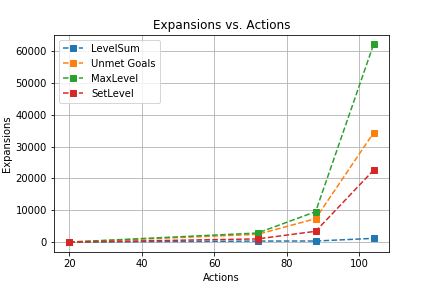
\includegraphics[width=0.5\columnwidth]{fig/results_034.png}
\caption{Search Method GBFGS w. SetLevel}
\end{center}
\label{fig034}
\end{figure}
        

\subsection{Greedy Best First Graph Search with SetLevel}

\begin{figure}[htpb]
\begin{center}
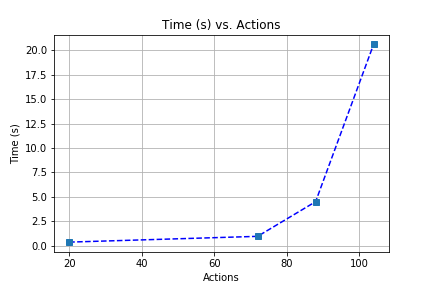
\includegraphics[width=0.5\columnwidth]{fig/results_031.png}
\caption{Search Method GBFGS w. SetLevel}
\end{center}
\label{fig031}
\end{figure}
        

\subsection{Greedy Best First Graph Search with LevelSum}

\begin{figure}[htpb]
\begin{center}
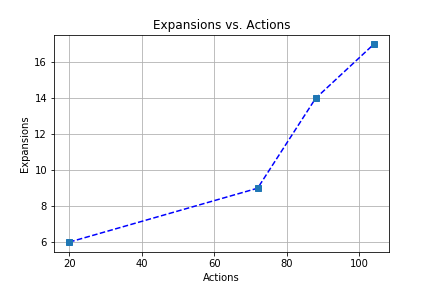
\includegraphics[width=0.5\columnwidth]{fig/results_134.png}
\caption{Search Method GBFGS w. LevelSum}
\end{center}
\label{fig134}
\end{figure}
        

\subsection{Greedy Best First Graph Search with LevelSum}

\begin{figure}[htpb]
\begin{center}
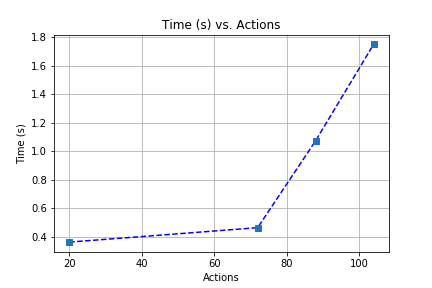
\includegraphics[width=0.5\columnwidth]{fig/results_131.png}
\caption{Search Method GBFGS w. LevelSum}
\end{center}
\label{fig131}
\end{figure}
        

\subsection{Greedy Best First Graph Search with MaxLevel}

\begin{figure}[htpb]
\begin{center}
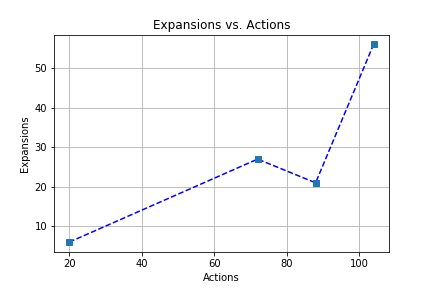
\includegraphics[width=0.5\columnwidth]{fig/results_234.png}
\caption{Search Method GBFGS w. MaxLevel}
\end{center}
\label{fig234}
\end{figure}
        

\subsection{Greedy Best First Graph Search with MaxLevel}

\begin{figure}[htpb]
\begin{center}
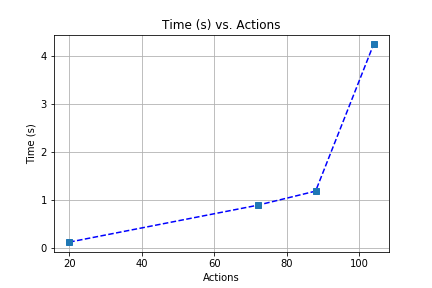
\includegraphics[width=0.5\columnwidth]{fig/results_231.png}
\caption{Search Method GBFGS w. MaxLevel}
\end{center}
\label{fig231}
\end{figure}
        

\subsection{Greedy Best First Graph Search with Unmet Goals}

\begin{figure}[htpb]
\begin{center}
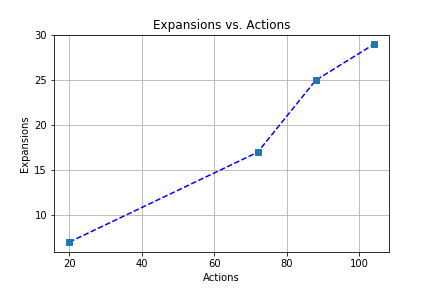
\includegraphics[width=0.5\columnwidth]{fig/results_334.png}
\caption{Search Method GBFGS w. Unmet Goals}
\end{center}
\label{fig334}
\end{figure}
        

\subsection{Greedy Best First Graph Search with Unmet Goals}

\begin{figure}[htpb]
\begin{center}
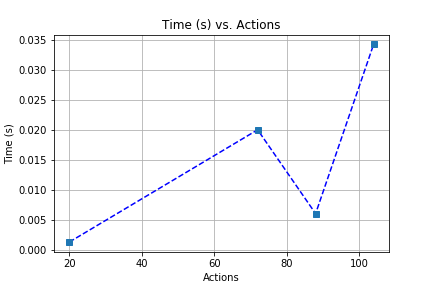
\includegraphics[width=0.5\columnwidth]{fig/results_331.png}
\caption{Search Method GBFGS w. Unmet Goals}
\end{center}
\label{fig331}
\end{figure}
        

\subsection{Uniform Cost Search}

\begin{figure}[htpb]
\begin{center}
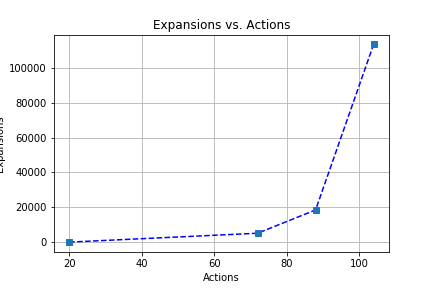
\includegraphics[width=0.5\columnwidth]{fig/results_434.png}
\caption{Search Method UCS}
\end{center}
\label{fig434}
\end{figure}
        

\subsection{Uniform Cost Search}

\begin{figure}[htpb]
\begin{center}
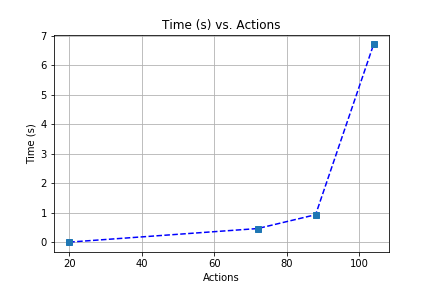
\includegraphics[width=0.5\columnwidth]{fig/results_431.png}
\caption{Search Method UCS}
\end{center}
\label{fig431}
\end{figure}
        

\subsection{Depth First Graph Search}

\begin{figure}[htpb]
\begin{center}
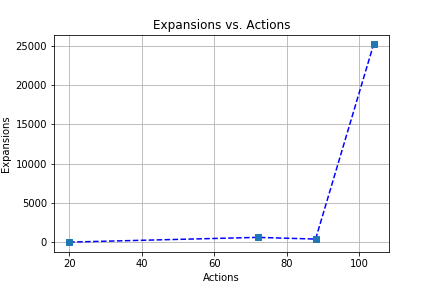
\includegraphics[width=0.5\columnwidth]{fig/results_534.png}
\caption{Search Method DFGS}
\end{center}
\label{fig534}
\end{figure}
        

\subsection{Depth First Graph Search}

\begin{figure}[htpb]
\begin{center}
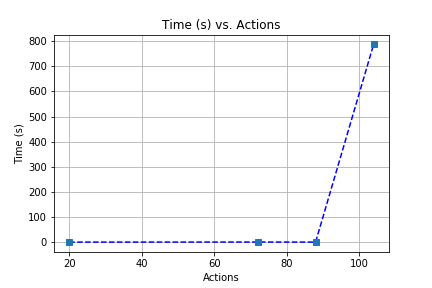
\includegraphics[width=0.5\columnwidth]{fig/results_531.png}
\caption{Search Method DFGS}
\end{center}
\label{fig531}
\end{figure}
        

\subsection{A* Search with SetLevel}

\begin{figure}[htpb]
\begin{center}
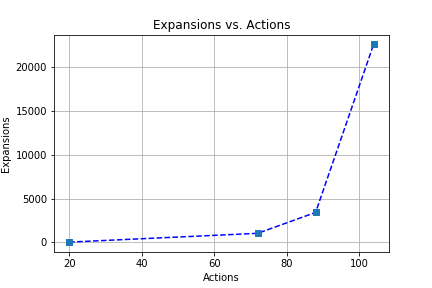
\includegraphics[width=0.5\columnwidth]{fig/results_634.png}
\caption{Search Method AS w. SetLevel}
\end{center}
\label{fig634}
\end{figure}
        

\subsection{A* Search with SetLevel}

\begin{figure}[htpb]
\begin{center}
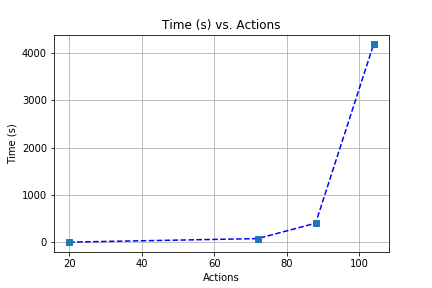
\includegraphics[width=0.5\columnwidth]{fig/results_631.png}
\caption{Search Method AS w. SetLevel}
\end{center}
\label{fig631}
\end{figure}
        

\subsection{A* Search with LevelSum}

\begin{figure}[htpb]
\begin{center}
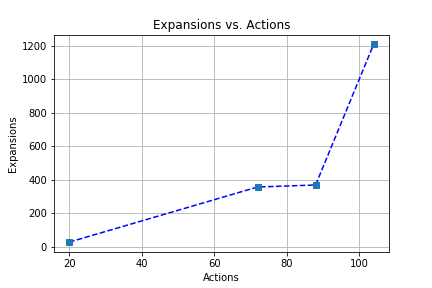
\includegraphics[width=0.5\columnwidth]{fig/results_734.png}
\caption{Search Method AS w. LevelSum}
\end{center}
\label{fig734}
\end{figure}
        

\subsection{A* Search with LevelSum}

\begin{figure}[htpb]
\begin{center}
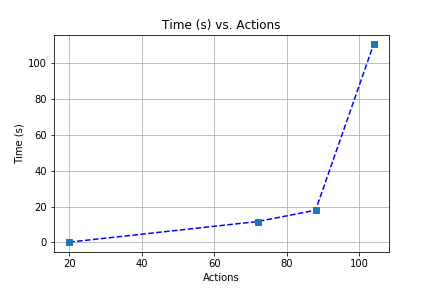
\includegraphics[width=0.5\columnwidth]{fig/results_731.png}
\caption{Search Method AS w. LevelSum}
\end{center}
\label{fig731}
\end{figure}
        

\subsection{A* Search with MaxLevel}

\begin{figure}[htpb]
\begin{center}
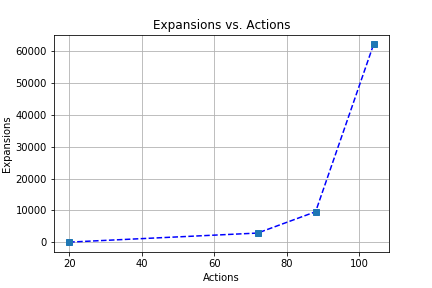
\includegraphics[width=0.5\columnwidth]{fig/results_834.png}
\caption{Search Method AS w. MaxLevel}
\end{center}
\label{fig834}
\end{figure}
        

\subsection{A* Search with MaxLevel}

\begin{figure}[htpb]
\begin{center}
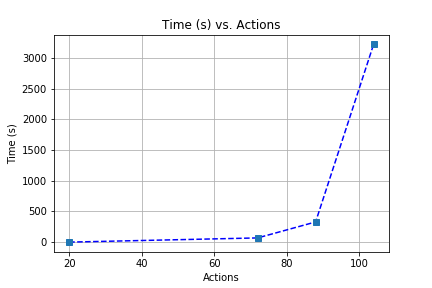
\includegraphics[width=0.5\columnwidth]{fig/results_831.png}
\caption{Search Method AS w. MaxLevel}
\end{center}
\label{fig831}
\end{figure}
        

\subsection{A* Search with Unmet Goals}

\begin{figure}[htpb]
\begin{center}
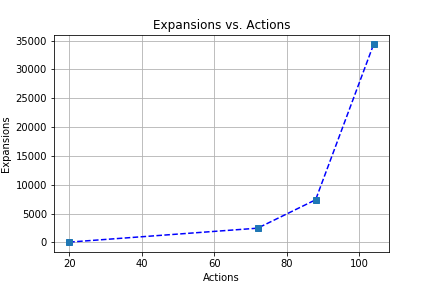
\includegraphics[width=0.5\columnwidth]{fig/results_934.png}
\caption{Search Method AS w. Unmet Goals}
\end{center}
\label{fig934}
\end{figure}
        

\subsection{A* Search with Unmet Goals}

\begin{figure}[htpb]
\begin{center}
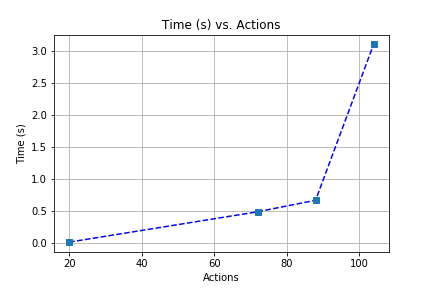
\includegraphics[width=0.5\columnwidth]{fig/results_931.png}
\caption{Search Method AS w. Unmet Goals}
\end{center}
\label{fig931}
\end{figure}
        

\subsection{Breadth First Search}

\begin{figure}[htpb]
\begin{center}
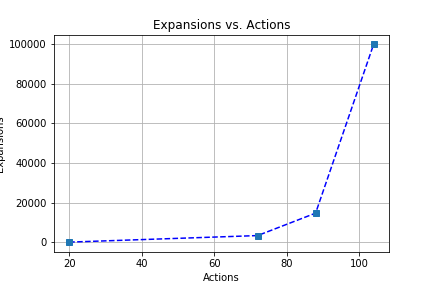
\includegraphics[width=0.5\columnwidth]{fig/results_1034.png}
\caption{Search Method BFS}
\end{center}
\label{fig1034}
\end{figure}
        

\subsection{Breadth First Search}

\begin{figure}[htpb]
\begin{center}
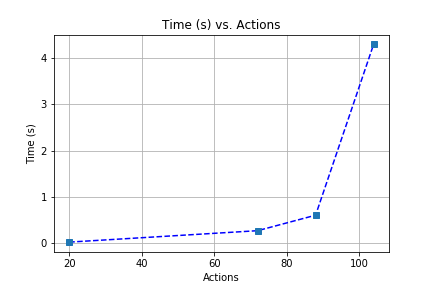
\includegraphics[width=0.5\columnwidth]{fig/results_1031.png}
\caption{Search Method BFS}
\end{center}
\label{fig1031}
\end{figure}

\subsection{Search Method vs. Plan length}

\begin{table}[htpb]
    \caption{ Air Cargo Problem 1 }
    \centering
    \begin{tabular}{ l | c }
    Search Method & Plan length \\ \hline 
BFS & 9 \\
DFGS & 619 \\
UCS & 9 \\
GBFGS w. Unmet Goals & 9 \\
GBFGS w. LevelSum & 9 \\
GBFGS w. MaxLevel & 9 \\
GBFGS w. SetLevel & 9 \\
AS w. Unmet Goals & 9 \\
AS w. LevelSum & 9 \\
AS w. MaxLevel & 9 \\
AS w. SetLevel & 9
\end{tabular}
    \label{airps1}
    \end{table}

    
\begin{table}[htpb]
    \caption{ Air Cargo Problem 2 }
    \centering
    \begin{tabular}{ l | c }
    Search Method & Plan length \\ \hline 
BFS & 14 \\
DFGS & 24132 \\
UCS & 14 \\
GBFGS w. Unmet Goals & 18 \\
GBFGS w. LevelSum & 17 \\
GBFGS w. MaxLevel & 17 \\
GBFGS w. SetLevel & 23 \\
AS w. Unmet Goals & 14 \\
AS w. LevelSum & 15 \\
AS w. MaxLevel & 14 \\
AS w. SetLevel & 14
\end{tabular}
    \label{airps2}
    \end{table}

    
\begin{table}[htpb]
    \caption{ Air Cargo Problem 3 }
    \centering
    \begin{tabular}{ l | c }
    Search Method & Plan length \\ \hline 
BFS & 6 \\
DFGS & 20 \\
UCS & 6 \\
GBFGS w. Unmet Goals & 6 \\
GBFGS w. LevelSum & 6 \\
GBFGS w. MaxLevel & 6 \\
GBFGS w. SetLevel & 6 \\
AS w. Unmet Goals & 6 \\
AS w. LevelSum & 6 \\
AS w. MaxLevel & 6 \\
AS w. SetLevel & 6
\end{tabular}
    \label{airps3}
    \end{table}

    
\begin{table}[htpb]
    \caption{ Air Cargo Problem 4 }
    \centering
    \begin{tabular}{ l | c }
    Search Method & Plan length \\ \hline 
BFS & 12 \\
DFGS & 392 \\
UCS & 12 \\
GBFGS w. Unmet Goals & 15 \\
GBFGS w. LevelSum & 14 \\
GBFGS w. MaxLevel & 13 \\
GBFGS w. SetLevel & 17 \\
AS w. Unmet Goals & 12 \\
AS w. LevelSum & 12 \\
AS w. MaxLevel & 12 \\
AS w. SetLevel & 12
\end{tabular}
    \label{airps4}
    \end{table}

    

\section{Conclusion}
t

\bibliographystyle{IEEEtran}
\bibliography{bibliography.bib}
\end{document}